\section{Porównanie z~wersją prototypową}
\indent

W celu porównania działania implementacji w środowisku \textrm{MATLAB} a tej w
\textit{C++}, przefiltrowany został przykładowy sygnał (MIT-BIH 100 próbki
1-250) przy użyciu obu implementacji. Na rysynkach \ref{rys:comp_d1} oraz
\ref{rys:comp_d2} przedstawiono przykładowe wyniki filtracji sygnału EKG,
odpowiednio dla usuniętego 1 i 2-óch IMF-ów.

\begin{figure}[!htb]
    \begin{center}
        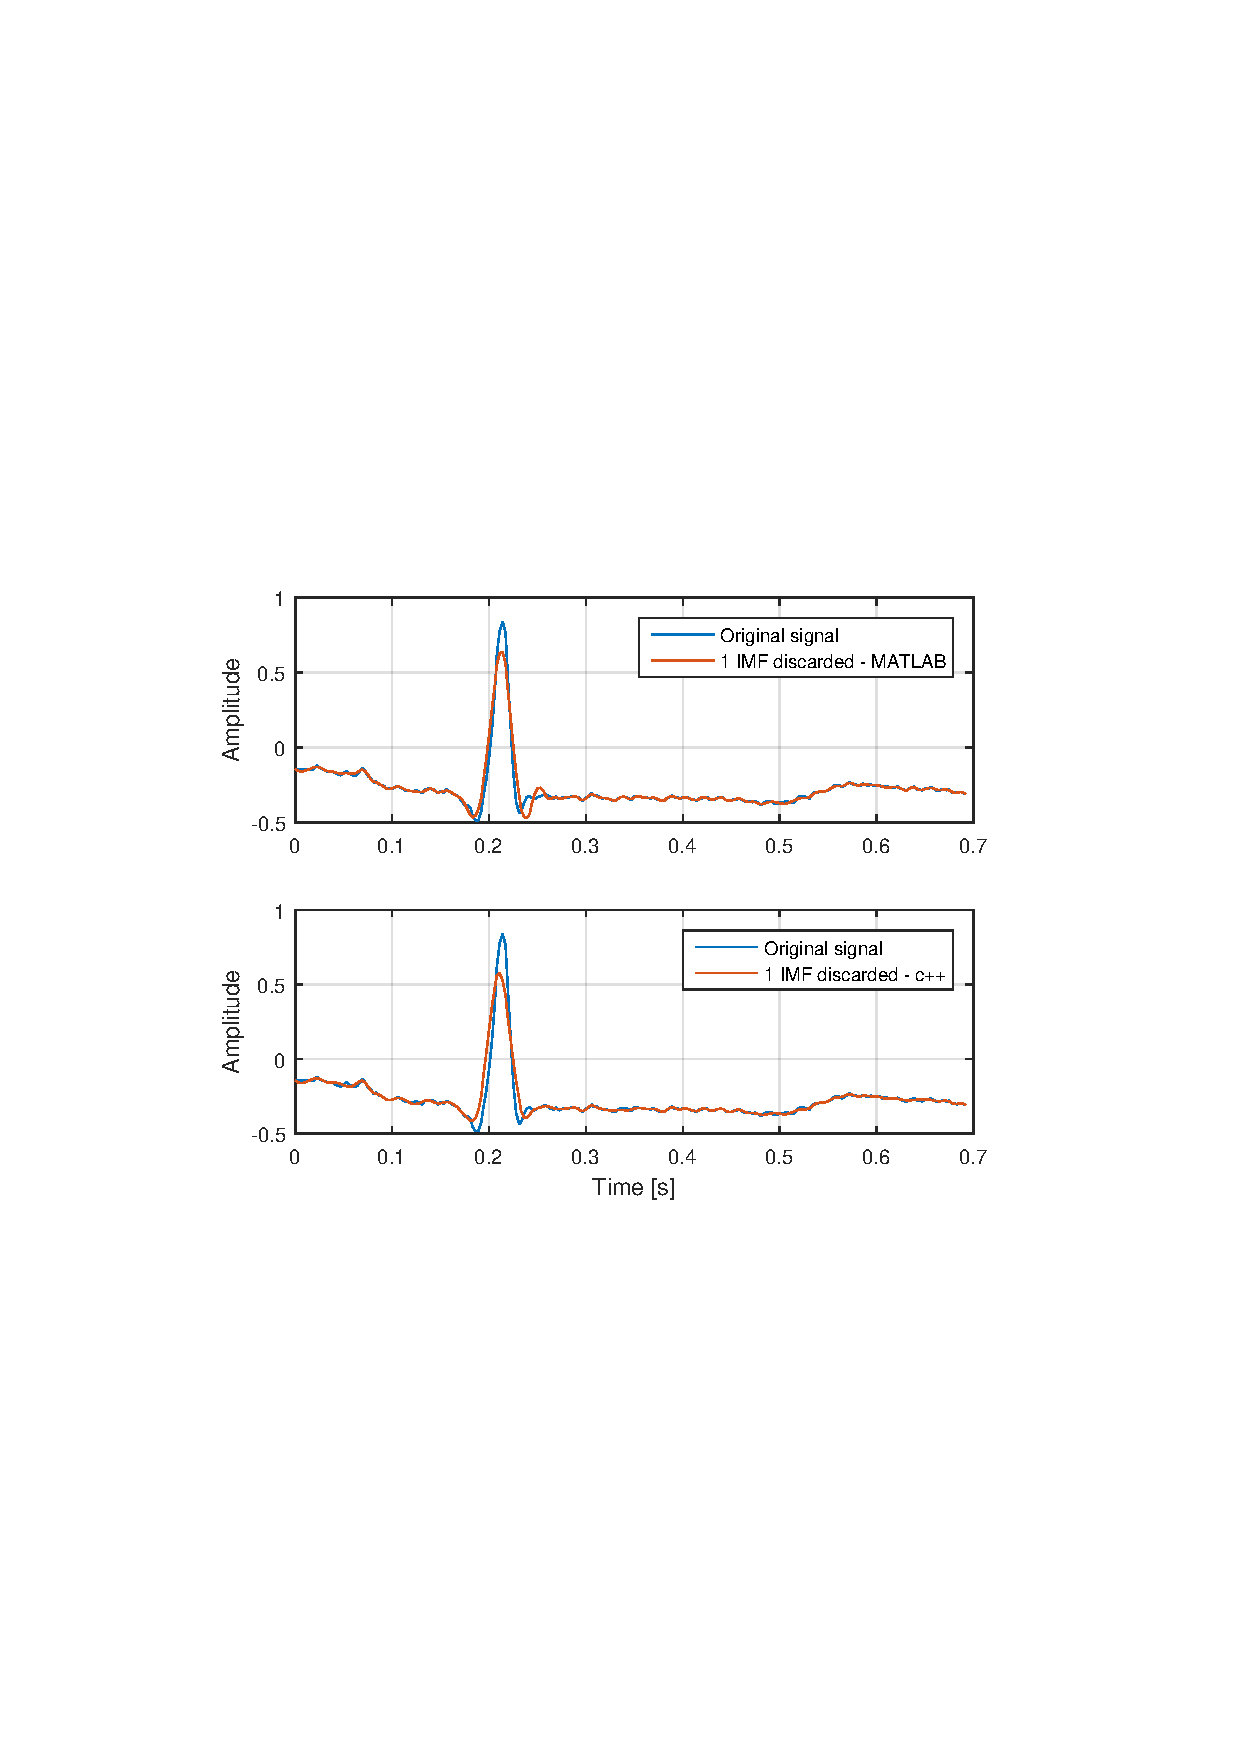
\includegraphics[width=14cm,trim=4cm 9cm 4cm 9cm,clip]
        {../img/mat_cpp_domp_d1.pdf}
    \end{center}
    \caption{Porównanie działania filtracji implementacji \textrm{MATLAB} i
    \textit{C++} przy odrzuceniu 1 IMF-a (Czas wykonania: \textrm{MATLAB} : 1534
    [ms], \textit{C++}: 126 [ms])}
    \label{rys:comp_d1}
\end{figure}

Gołym okiem widać różnice sygnałów przefiltrowanych dwoma implementacjami, zatem
zostały poddane one głębszej analizie.

W jej wyniku odnaleziono przyczynę różnic
wyników w badanych implementacjach. Są one spowodowane przez inne wyniki
wyznaczania funkcji sklejanych w pakietach \textrm{MATLAB} i \textit{Eigen}.
Przykładowe porównanie na przykładzie górnej obwiedni w pierwszej iteracji
algorytmu \textit{emd}, dla sygnału użytego przy porównaniach, znajduje się na
rysunku \ref{rys:comp_spline}.

\newpage

\begin{figure}[!htb]
    \begin{center}
        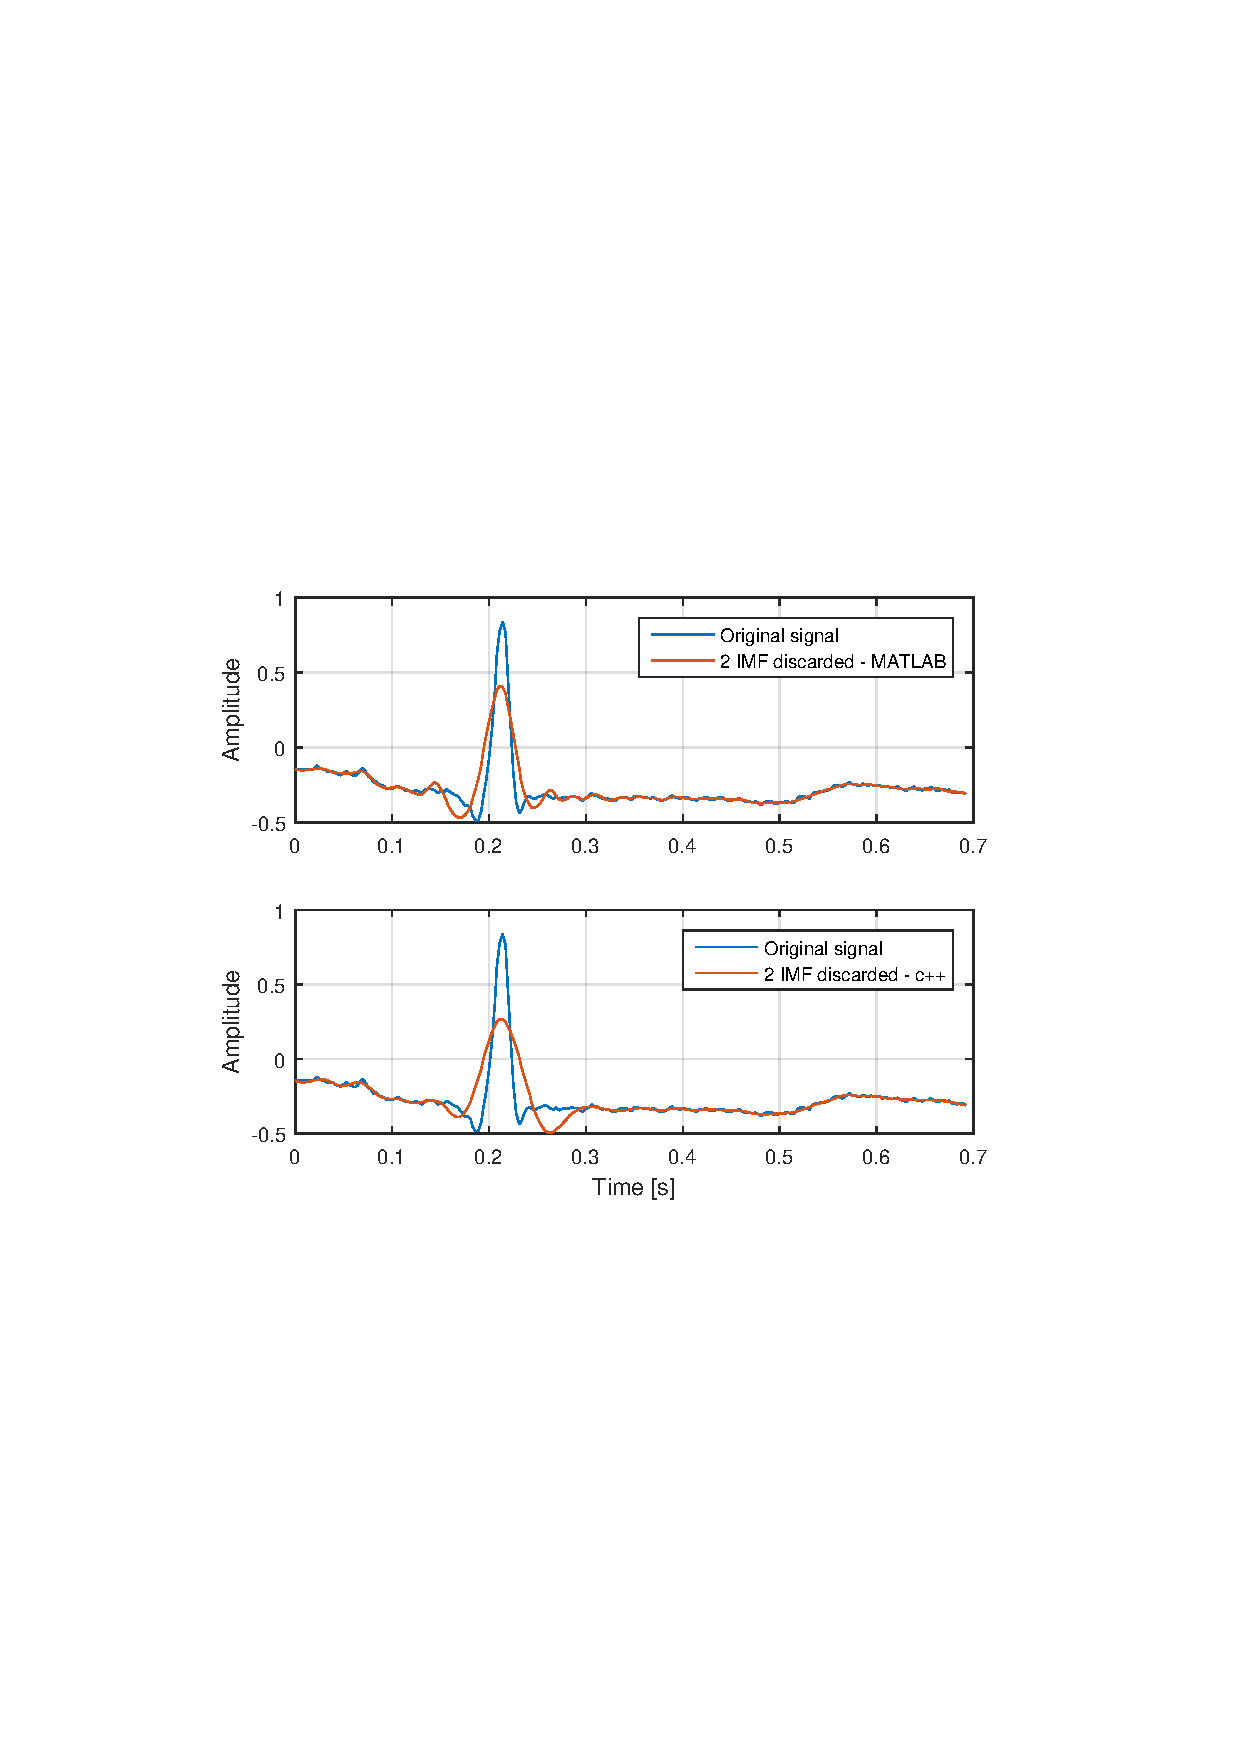
\includegraphics[width=13cm,trim=4cm 9.5cm 4cm 10cm,clip]
        {../img/mat_cpp_domp_d2.pdf}
    \end{center}
    \caption{Porównanie działania filtracji implementacji \textrm{MATLAB} i
    \textit{C++} przy odrzuceniu 2 IMF-ów (Czas wykonania: \textrm{MATLAB} :
    1523 [ms], \textit{C++}: 130 [ms])}
    \label{rys:comp_d2}
\end{figure}

\begin{figure}[!htb]
    \begin{center}
        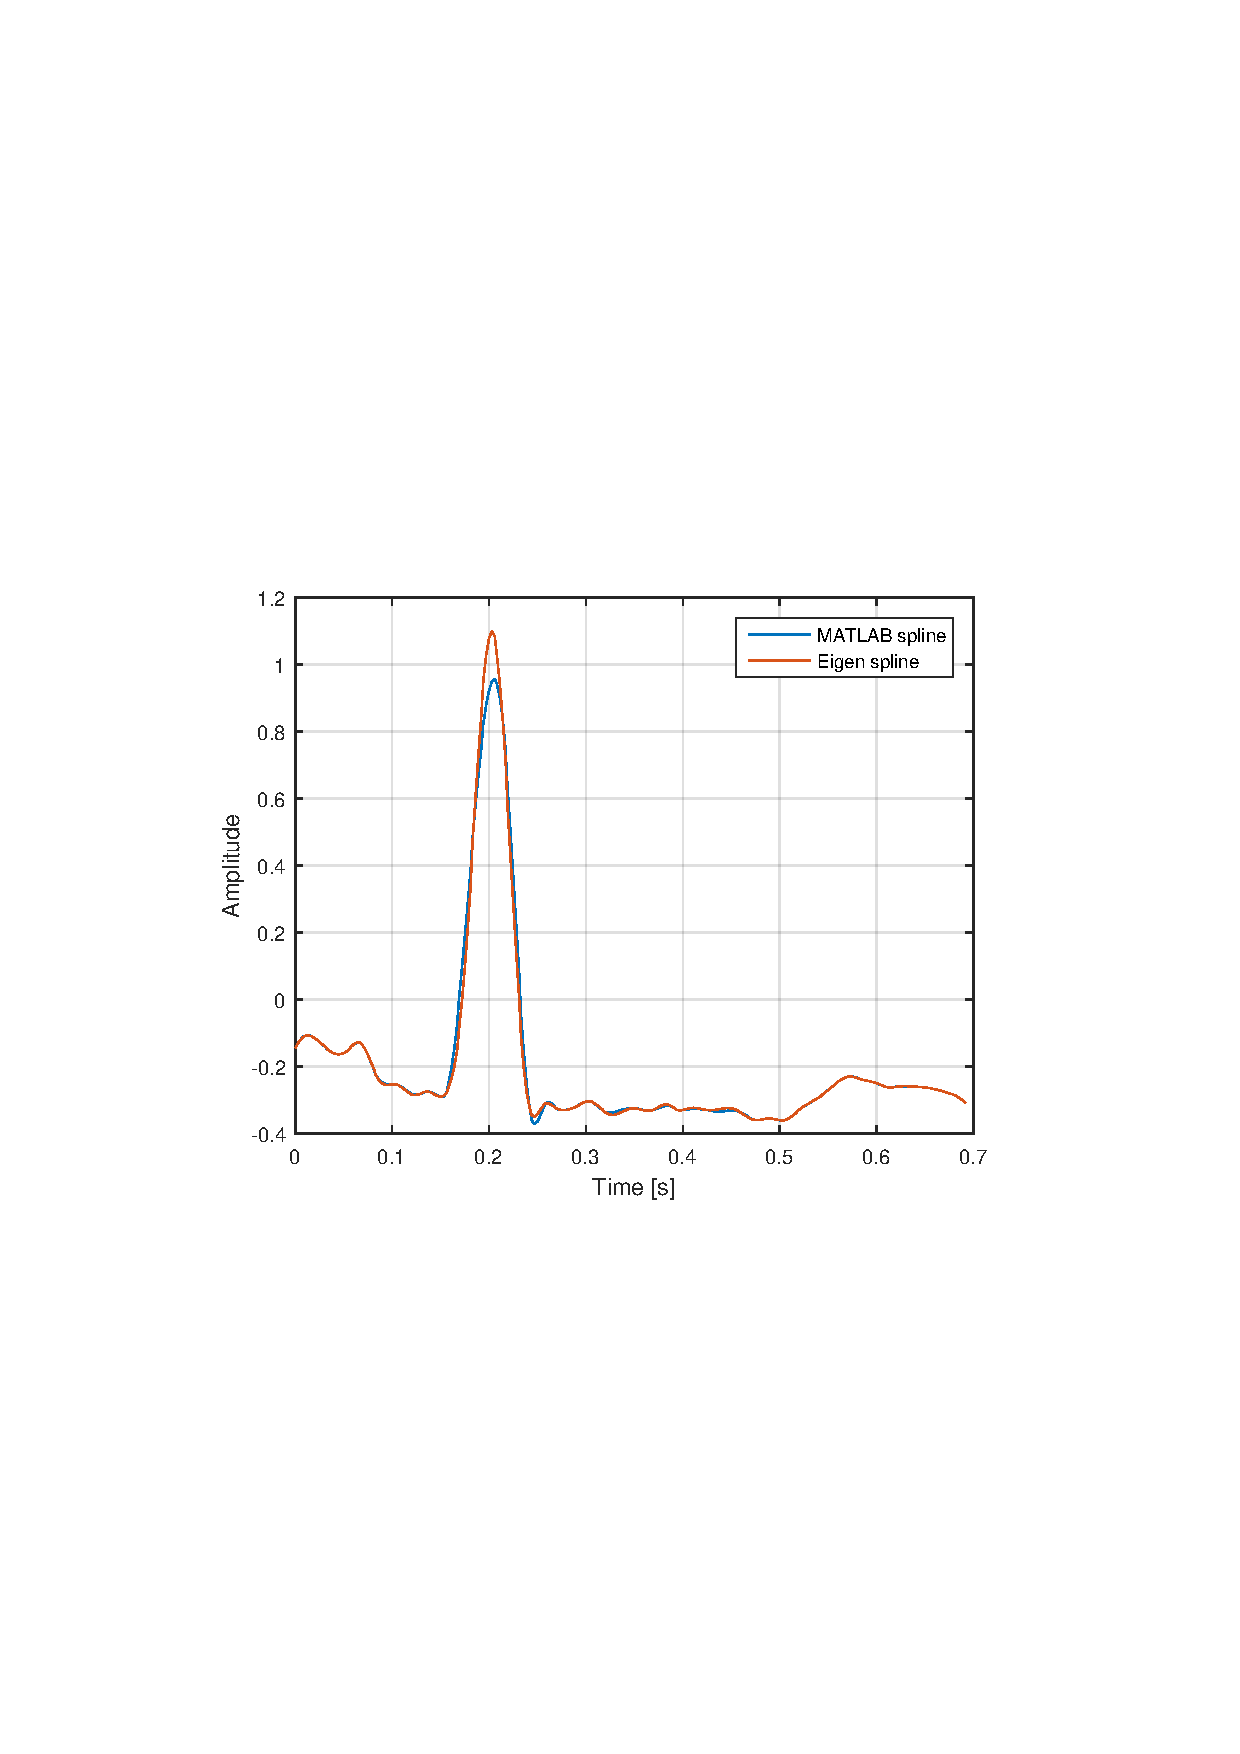
\includegraphics[width=13cm,trim=4cm 9.5cm 4cm 10cm,clip]
        {../img/spline_comp.pdf}
    \end{center}
    \caption{Porównanie implementacji spline-ów pakietów \textit{Eigen} oraz
    \textrm{MATLAB}}
    \label{rys:comp_spline}
\end{figure}

\newpage

\section{Analiza jakości filtracji}
\indent

W celu wyznaczenia jakichkolwiek wskaźników jakości, potrzebne są sygnały
referencyjne, nie posiadające szumów, oraz ich zaszumione odpowiedniki. Na
potrzeby analizy jakości algorytmu został wygenerowany sygnał sinusoidalny
zaszumiony zmienną losową o jednostajnym rozkładzie, generującą liczby z zakresu
(-0.1,0.1). Użyty do porównań wskaźnik to RMSE, który obliczony został na
podstawie równania \eqref{equ:rmse}, gdzie $x$ to badany sygnał, a
$\overline{x}$ to sygnał referencyjny. RMSE zaszumionego sygnału wynosi
$0.0034$.

\begin{equation}
    RMSE = \frac{1}{N-1}\sum_{i=1}^{N}(x_i-\overline{x_i})
    \label{equ:rmse}
\end{equation}

\begin{figure}[!htb]
    \begin{center}
        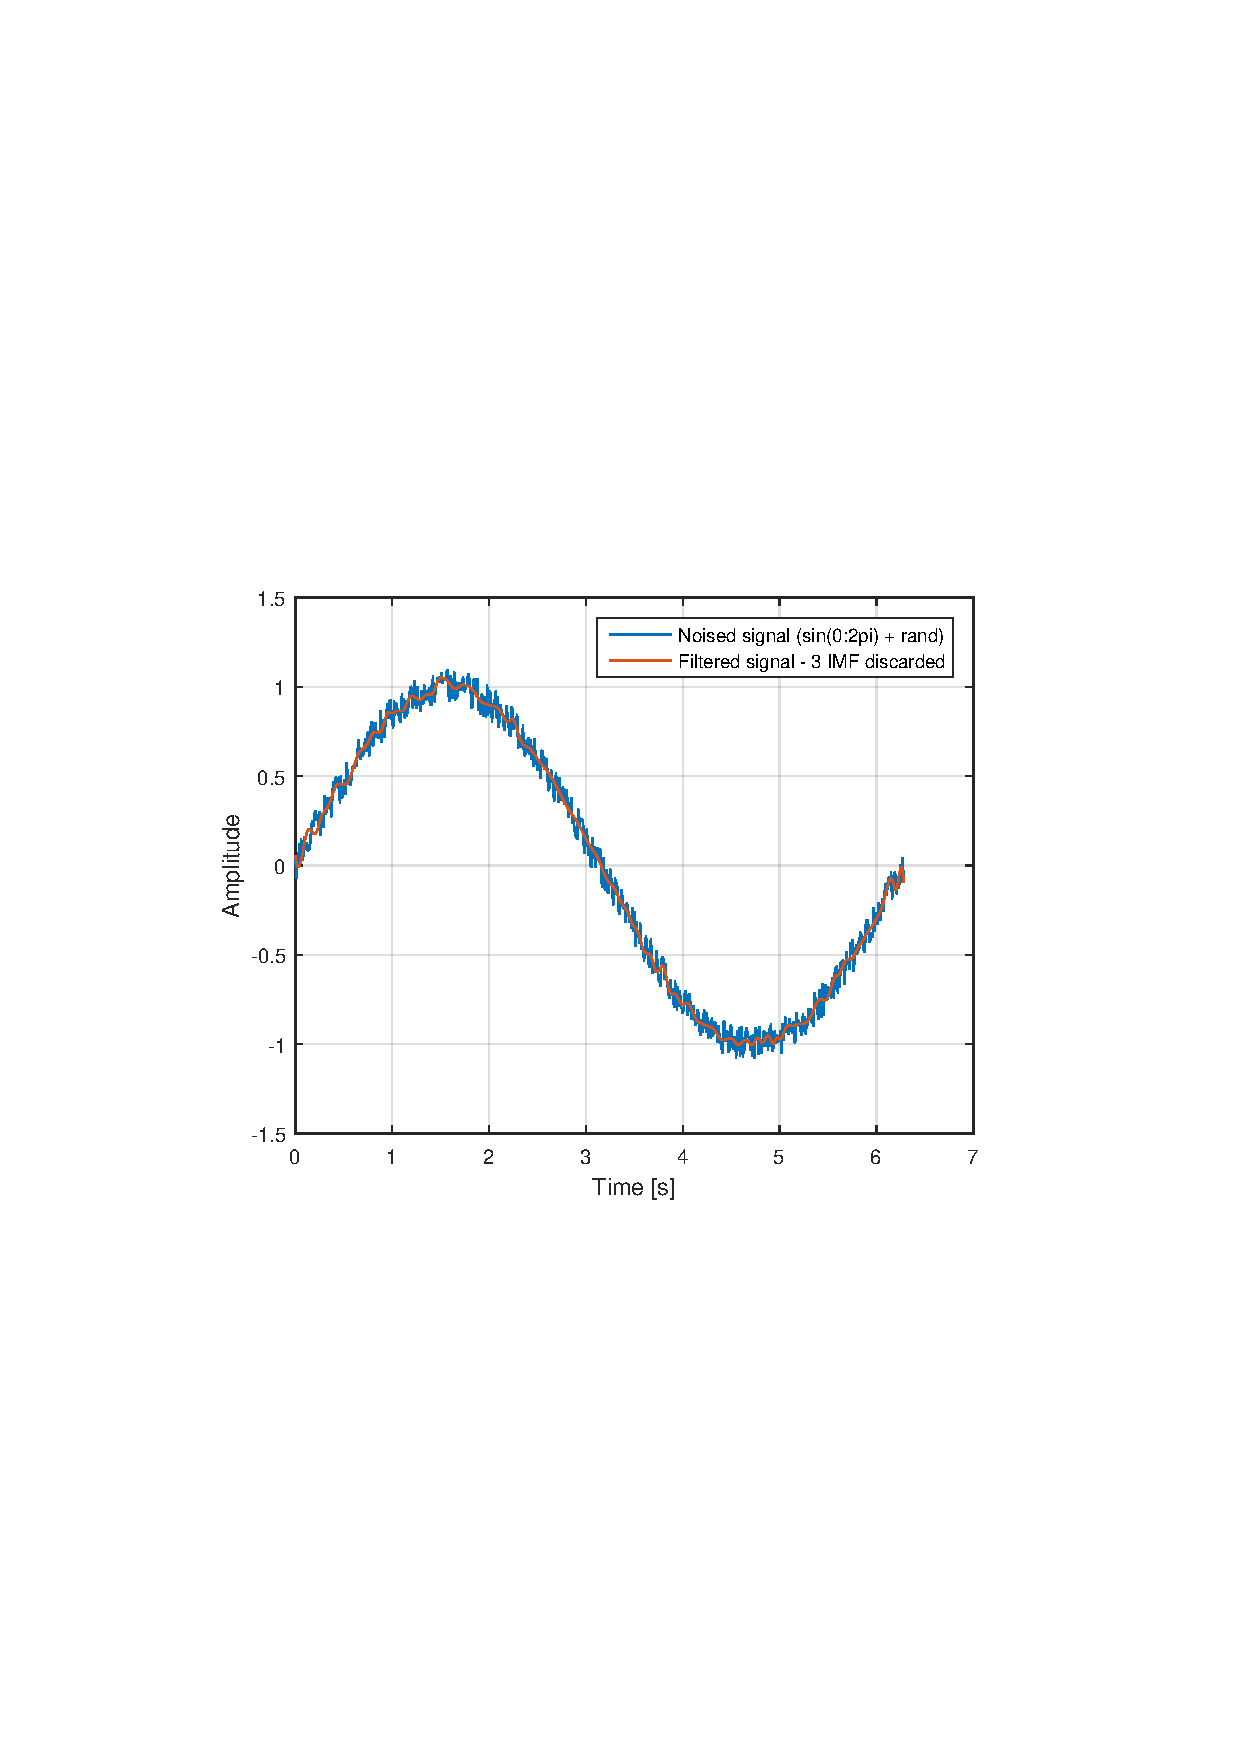
\includegraphics[width=13cm,trim=4cm 9cm 4cm 9cm,clip]
        {../img/sin_rmse3.pdf}
    \end{center}
    \caption{Sygnał referencyjny dla usuniętych 3 IMF-ów (RMSE = $0.00048$)}
    \label{rys:sin_rmse3}
\end{figure}

\newpage

\begin{figure}[!htb]
    \begin{center}
        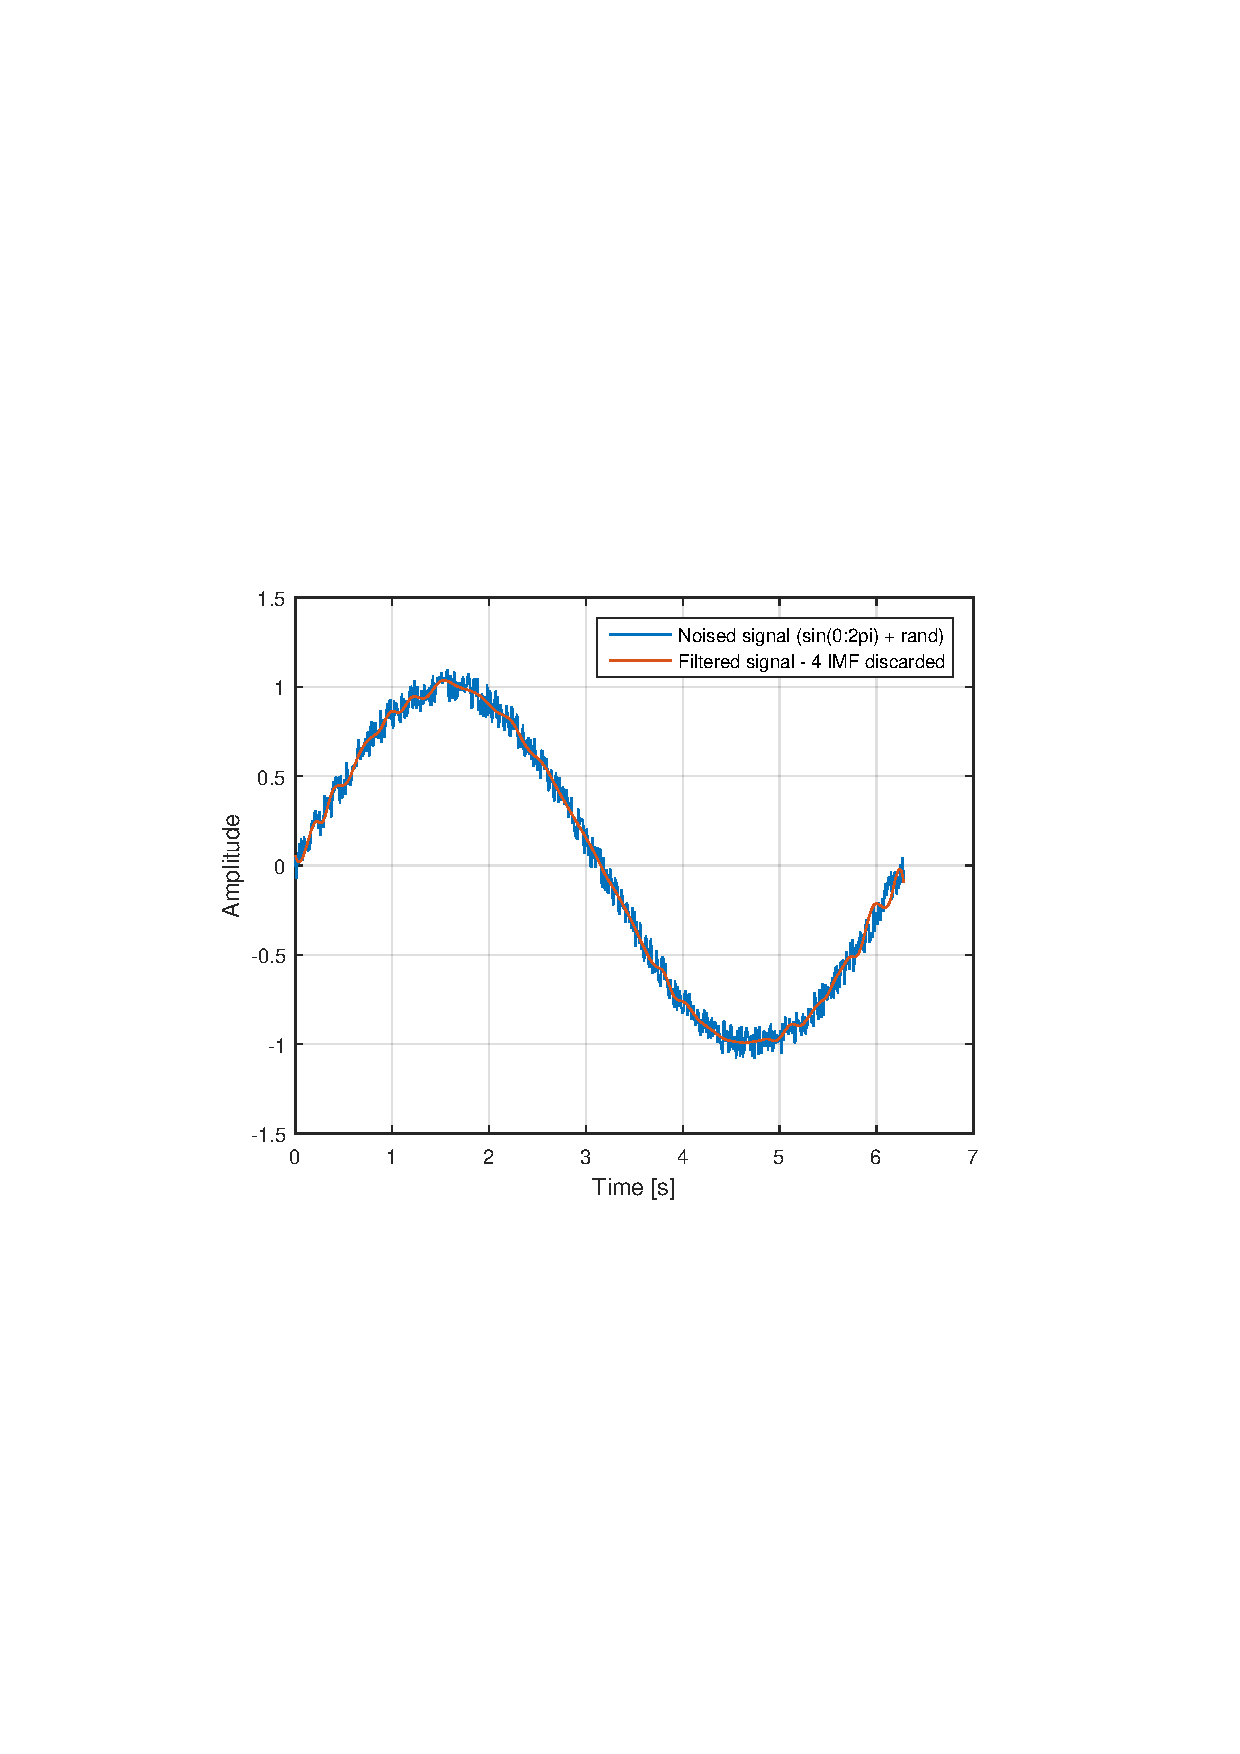
\includegraphics[width=13cm,trim=4cm 9.5cm 4cm 10cm,clip]
        {../img/sin_rmse4.pdf}
    \end{center}
    \caption{Sygnał referencyjny dla usuniętych 4 IMF-ów (RMSE = $0.00045$)}
    \label{rys:sin_rmse4}
\end{figure}

\begin{figure}[!htb]
    \begin{center}
        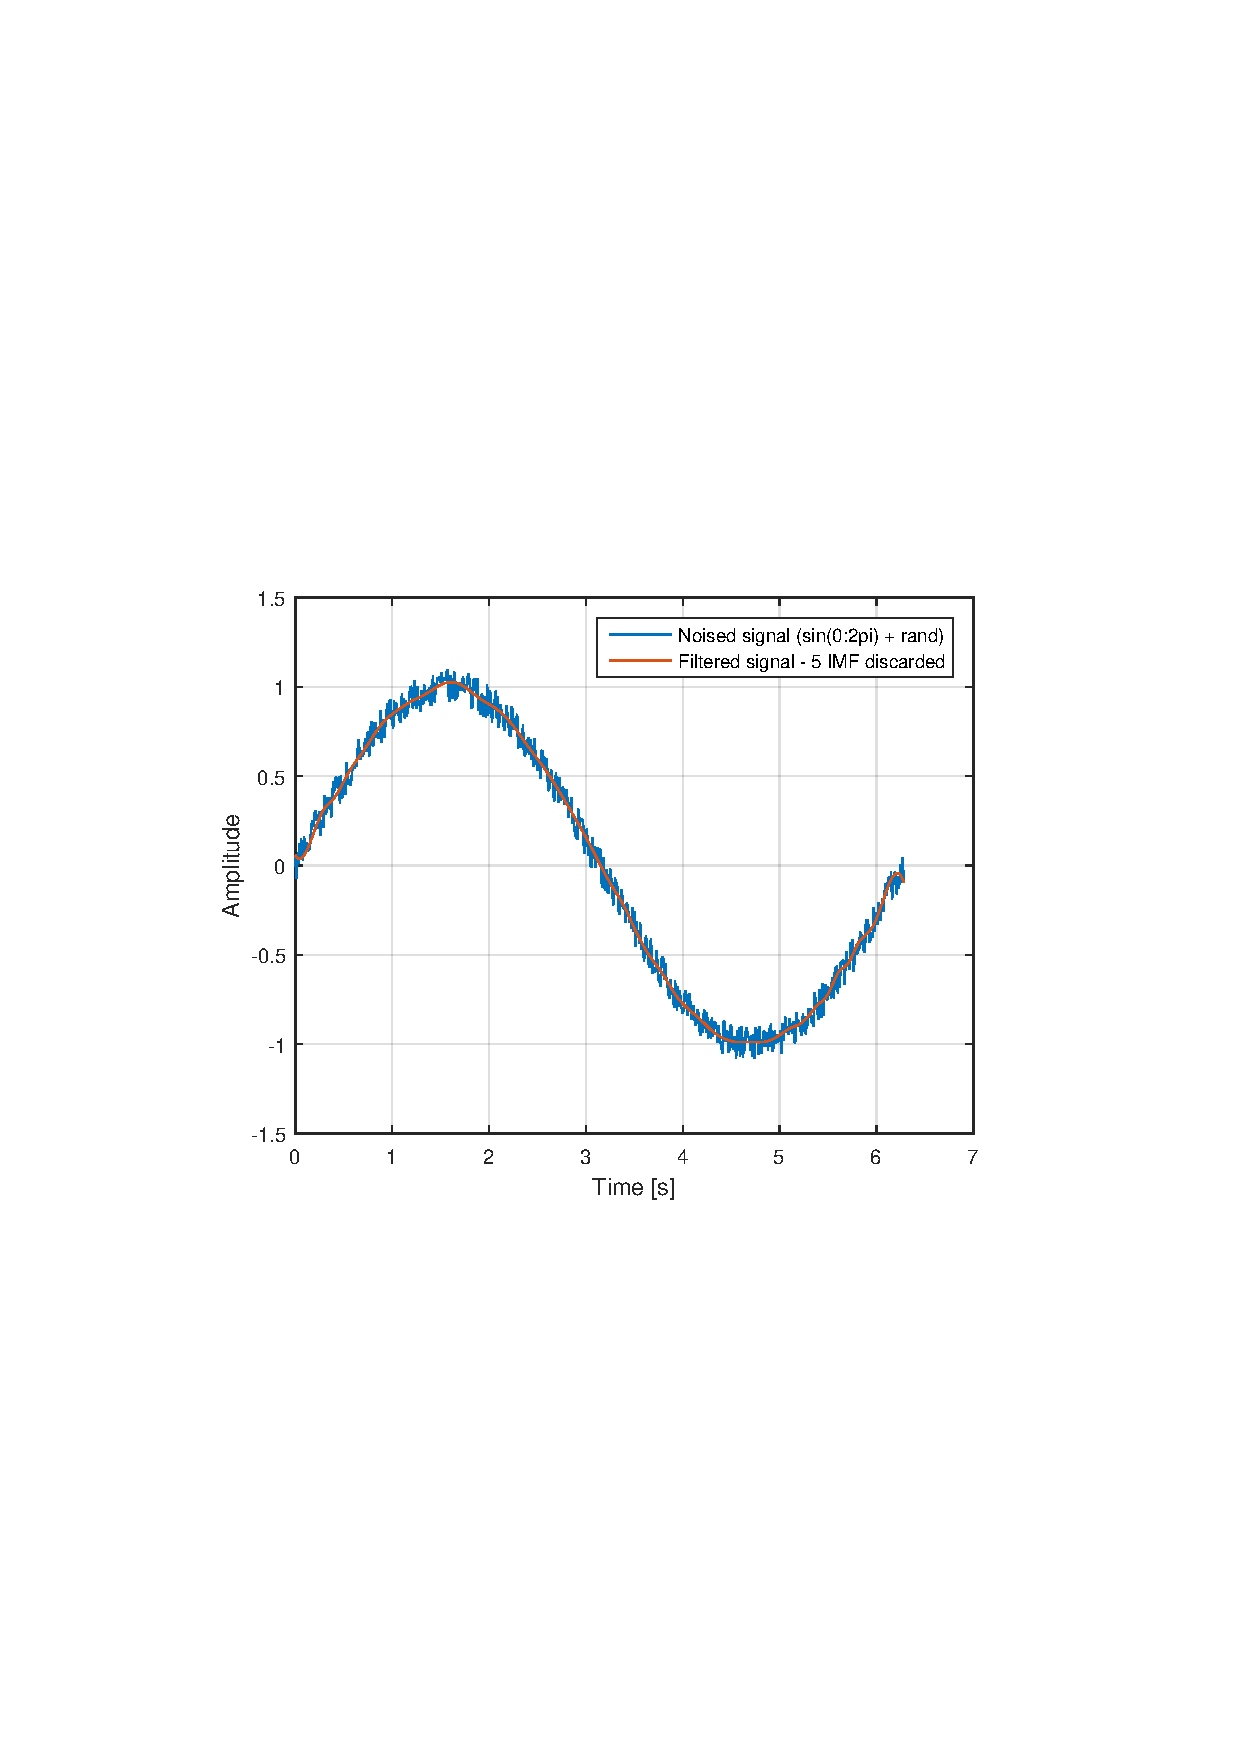
\includegraphics[width=13cm,trim=4cm 9.5cm 4cm 10cm,clip]
        {../img/sin_rmse5.pdf}
    \end{center}
    \caption{Sygnał referencyjny dla usuniętych 5 IMF-ów (RMSE = $0.00021$)}
    \label{rys:sin_rmse5}
\end{figure}
